% NEUTRONICS BEAMER TEMPLATE -- START EDITING IN LINE 90
%\documentclass[xcolor=x11names, compress, handout]{beamer}
\documentclass[xcolor=x11names, compress]{beamer}
\usepackage{pgfpages}
\usefonttheme[onlymath]{serif}
\setbeamerfont{caption}{size=\scriptsize}
\setbeameroption{show notes on second screen=right}
%\setbeameroption{hide notes}

\definecolor{CoolBlack}{rgb}{0.0, 0.18, 0.39}
\definecolor{byellow}{rgb}{0.55037, 0.38821, 0.06142}

\usepackage[T1]{fontenc}
\usepackage[utf8]{inputenc}
\usepackage{lmodern}
\usepackage{amsthm}
\usepackage{amssymb}
\usepackage{amstext}
\usepackage{bm}
\usepackage{graphicx}
\usepackage{epstopdf}
\usepackage{amsmath}
\usepackage{setspace}
\usepackage{tikz}
\usepackage{Tabbing}
\usepackage{mathrsfs}
\usepackage[mathcal]{euscript}
\usepackage{epsfig}
\usepackage{changepage}
\usepackage{xcolor}
\usepackage{fancyvrb}
\usepackage{caption}
\usepackage{color}
\usepackage[version=3]{mhchem}
\usepackage{hyperref}
\usepackage{multirow}
%\usepackage[firstpage]{draftwatermark}
\usepackage{animate}
\usepackage{appendixnumberbeamer}



\usetikzlibrary{decorations.fractals}

\setbeamerfont{title like}{shape=\scshape}
\setbeamerfont{frametitle}{shape=\scshape}

\setbeamercolor*{lower separation line head}{bg=CoolBlack}
\setbeamercolor*{normal text}{fg=black,bg=white}
\setbeamercolor*{alerted text}{fg=dgreen} 
\setbeamercolor*{example text}{fg=black}
\setbeamercolor*{structure}{fg=black}

% Margins
\mode<presentation>
{
  \definecolor{berkeleyblue}{HTML}{003262}
  \definecolor{berkeleygold}{HTML}{FDB515}
  \usetheme{Boadilla}      % or try Darmstadt, Madrid, Warsaw, Boadilla...
  %\usecolortheme{dove} % or try albatross, beaver, crane, ...
  \setbeamercolor{structure}{fg=berkeleyblue,bg=berkeleygold}
  \setbeamercolor{palette primary}{fg=berkeleyblue,bg=berkeleygold}
  \setbeamercolor{palette secondary}{fg=berkeleyblue,bg=berkeleygold}
  \setbeamercolor{palette tertiary}{bg=berkeleyblue,fg=white}
  \usefonttheme{structurebold}  % or try serif, structurebold, ...
  \useinnertheme{circles}
  \setbeamertemplate{caption}[numbered]
  \usebackgroundtemplate{}
}

%% Beamer Layout %%%%%%%%%%%%%%%%%%%%%%%%%%%%%
\useoutertheme[subsection=false,shadow]{miniframes}
%\useinnertheme{default}
%\usefonttheme{serif}
%\usepackage{palatino}
%\usepackage{tabu}
% addition of color
\definecolor{dgreen}{rgb}{0.,0.6,0.}
\definecolor{RawSienna}{cmyk}{0,0.72,1,0.45}
%\usepackage[sorting=none]{biblatex}
\mode<presentation>

% Links
\definecolor{links}{HTML}{003262}
\hypersetup{colorlinks,linkcolor=,urlcolor=links}

% columns
\renewcommand{\(}{\begin{columns}}
\renewcommand{\)}{\end{columns}}
\newcommand{\<}[1]{\begin{column}{#1}}
\renewcommand{\>}{\end{column}}

%%%%%%%%%%%%%%%%%%%%%%%%%%%%%%%%%%%%%%%%%%%%%%%%%%%%%%%%%%%%%%%%%%%%%%%%%%%%%%%%%%%%%%%%%%%%%%%%%%%%%%%%%%%%%%%%%%%%%%%%%%%%%%%%%%%%%%%%%%%%%%%%%%%%%%%%%

% START EDITING HERE

\setbeamertemplate{bibliography item}{\insertbiblabel}
% \setbeamertemplate{note page}{\pagecolor{yellow!5}\insertnote}
\usepackage{algorithm}
\usepackage{algpseudocode}
\usepackage{appendixnumberbeamer}
\usepackage{booktabs}
\usepackage{amsmath}
\usepackage{tikz}
\usepackage{xcolor}
\usepackage[super]{nth}
\usepackage{sty/commands}
\usepackage{appendixnumberbeamer}
\usepackage{hyperref}
\newcommand\Warning{%
 \makebox[1.4em][c]{%
 \makebox[0pt][c]{\raisebox{.1em}{\small!}}%
 \makebox[0pt][c]{\color{red}\Large$\bigtriangleup$}}}%
%THIS IS THE BEAR WATERMARK IN THE COVER SLIDE; YOU MAY EXCLUDE IT
%\SetWatermarkText{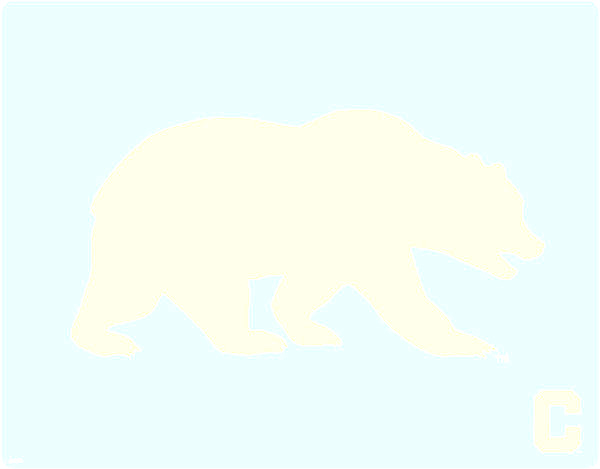
\includegraphics{0calbear.jpg}}
%\SetWatermarkAngle{0}
%\SetWatermarkScale{0.61}
%%%%%%%%%%%%%%%%%%%%%%

\AtBeginSection[]{
  \AtBeginSection[]
  {
     \begin{frame}[noframenumbering, plain]
     \frametitle{Outline}
     \tableofcontents[currentsection]
     \end{frame}
  }
  % \begin{frame}[noframenumbering, plain]
  % \vfill
  % \centering
  % \begin{beamercolorbox}[sep=8pt,center,shadow=true,rounded=true]{title}
  %   \usebeamerfont{title}\insertsectionhead\par%
  % \end{beamercolorbox}
  % \vfill
  % \end{frame}
}

%THIS IS THE INFO AT THE BOTTOM OF YOUR FRAMES
\title{Qualification Exam}
\author{J.S. Rehak}
\date{September \nth{4}, 2019}

%%%%%%%%%%%%%%%%%%%%%%%%%%%%%%%%%%%%%%%%%%%%%%%%%%

\begin{document}

%%%%%%%%%%%%%%%%%%%%%%%%%%%%%%%%%%%%%%%%%%%%%%%%%%%%%%
\begin{frame}[plain]
%THIS IS THE TITLE OF THE TALK
\title{BART\\\large{A new framework for developing and evaluating
  acceleration schemes for the neutron transport equation}}

%FEEL FREE TO EDIT THE COVER LAYOUT AS NEEDED
\author{
\begin{tabular}{c}
%YOUR NAME
J. S. Rehak\\
\vspace{10pt}\\
\includegraphics[height=2.5cm]{0bk.eps}
\end{tabular}}
\date{\vspace{-20pt}\\
  \begin{tabular}{c}
    \large{Qualification Exam} \\
 September \nth{4}, 2019
  \end{tabular}
}

\titlepage
\end{frame}

%----------------------------------------------------------%
% WHEN YOU START A NEW SECTION, IT WILL SHOW UP AS A CLICKABLE
% SHORTCUT AT THE TOP OF YOUR FRAMES

\begin{frame}
  \frametitle{Outline}
  \tableofcontents
\end{frame}

\section{\scshape Transport Equation}

\frame[c]{\frametitle{Steady-state Boltzman Transport Equation}

  Our problem of interest is the time-independent transport equation
  on a domain of interest $\rvec \in V$~\cite{lewis1993},
  
\begin{align*}
  &\left[ \oh\cdot  \nabla + \Sigma_t(\rvec,E) \right] \psi(\rvec,E,\oh)\\
  & \quad \quad \quad= \int_0^{\infty}dE'\int_{4\pi}d\oh'\Sigma_s(\rvec, E'\rightarrow E,\oh'\rightarrow\oh)
    \psi(\rvec,E',\oh') \\ & \quad \quad \quad+ Q(\psi, \rvec, E, \oh)\;,
\end{align*}
with a given boundary condition,
\begin{align*}
  \psi(\rvec,E,\oh) = \Gamma(\rvec, E, \oh), \quad \rvec \in \partial V,
  \quad \oh \cdot \hat{n} < 0
\end{align*}
}

\begin{frame}
  \frametitle{Iterative Solving Method}
  
  Assuming the source $Q$ is not a function of $\psi$,  we define the
  source-iteration iterative scheme for iteration $i$,

  \begin{align*}
  &\left[ \oh\cdot  \nabla + \Sigma_t(\rvec,E) \right] \alert<2>{\psi^{i+1}}(\rvec,E,\oh)\\
  & \quad \quad \quad= \int_0^{\infty}dE'\int_{4\pi}d\oh'\Sigma_s(\rvec, E'\rightarrow E,\oh'\rightarrow\oh)
    \alert<2>{\psi^{i}}(\rvec,E',\oh') \\ & \quad \quad \quad+ Q(\rvec, E, \oh)\;,
  \end{align*}

  with the same boundary condition and initial condition
  $\psi^0(\rvec, E, \oh)$.

  \onslide<3->{
  \begin{block}{Question}
    How does the error in our iterative solution $\psi^i$ evolve with time?
  \end{block}}
\end{frame}

\frame[c]{\frametitle{Error Analysis}
  \onslide<2->{
  Start with the single-energy, one
  dimension, infinite homogeneous medium with isotropic scattering.}
\onslide<2->{
  \begin{equation}
    \label{eq:single_energy}
    \left[\mu\frac{\partial}{\partial x} + \Sigma_t\right]\psi(x, \mu)
    = \frac{\Sigma_s}{2}\int_{-1}^{1}\psi(x, \mu')d\mu' +
    \frac{Q}{2}\;.
  \end{equation}}
\only<2>{
  \begin{equation*}
    \mu = \cos{\theta}
  \end{equation*}
  }
\onslide<3->{
  With source iteration scheme,}
\onslide<3->{
  \begin{equation}
        \label{eq:single_energy_iterative}
    \left[\mu\frac{\partial}{\partial x} + \Sigma_t\right]\psi^{i+1}(x, \mu) = \frac{\Sigma_s}{2}\int_{-1}^{1}\psi^i(x, \mu')d\mu' + \frac{Q}{2}\;.
  \end{equation}}
\onslide<4->{
Subtracting Eq.~\eqref{eq:single_energy_iterative} from
Eq.~\eqref{eq:single_energy} gives an equation for the iteration error,
\begin{equation*}
        \left[ \mu\frac{\partial}{\partial x} + \Sigma_t\right]\varepsilon^{i+1}(x, \mu) = \frac{\Sigma_s}{2}\int_{-1}^{1}\varepsilon^i(x, \mu')d\mu'\;.
       \end{equation*}}
  \note{
    \begin{itemize}
    \item How can we be sure that source iteration will converge? What
      controls the convergence rate? To determine this we can use a Fourier analysis.
    \item We need to start with a lot of assumptions to get a very
      simplified version of our transport equation.
    \item We define what we mean by error, and get an equation that
      relates the error in each step to the previous
      step. Unsurprisingly it looks like our original equation,
      because the evolution of the solution and the evolution of the
      error are related.
    \end{itemize}

    }
  }

\frame[c]{\frametitle{Fourier Analysis} To see how the error evolves
    in space with each iteration, we can use Fourier
    analysis~\cite{Adams2002}. \pause Let $\lambda$ define a spatial wavelength,
  \begin{equation*}
    \lambda = \frac{\ell}{n}, \quad \ell = \frac{1}{\Sigma_t}, \quad \forall n \in \mathbb{R}\;.
  \end{equation*}
  \pause
  With associated linear wave number,
  \begin{equation*}
    \lwn = \frac{1}{\lambda} = \frac{n}{\ell} = n \cdot \Sigma_t\;.
  \end{equation*}
  \pause
    Perform an inverse Fourier transform, expressing error in spatial
    frequency space,
    \begin{equation*}
      \varepsilon^i(x, \mu) = \int_{-\infty}^{\infty}\hat{\varepsilon}^i(n, \mu)e^{i\Sigma_t n x}dn\;.
    \end{equation*}


    \note{
      We can examine the modes of the spatial error by using an
        inverse Fourier transform. This will give us an idea of how
        the spatial frequencies of the error. We need to decide on an
        error wavelength, which gives us a linear error
        frequency. Higher $n$ means higher error frequency, with $n =
        0$ being infinite wavelength, completely non-coupled error.
        }
  }

\frame[c]{
  \frametitle{Fourier Analysis}
  After plugging into our equation for error and some rearranging,
  \begin{equation*}
    \int_{-1}^{1}\hat{\varepsilon}^{k+1}(n, \mu)d\mu = \Lambda(n)\int_{-1}^{1}\hat{\varepsilon}^{k}(n, \mu')d\mu'\;,
  \end{equation*}
  Where,
  \begin{equation*}
    \Lambda(n) = \frac{\Sigma_s}{\Sigma_t}\cdot \frac{\tan^{-1}{(n)}}{n}\;.
  \end{equation*}
\pause
  \begin{figure}[H]
    \centering
    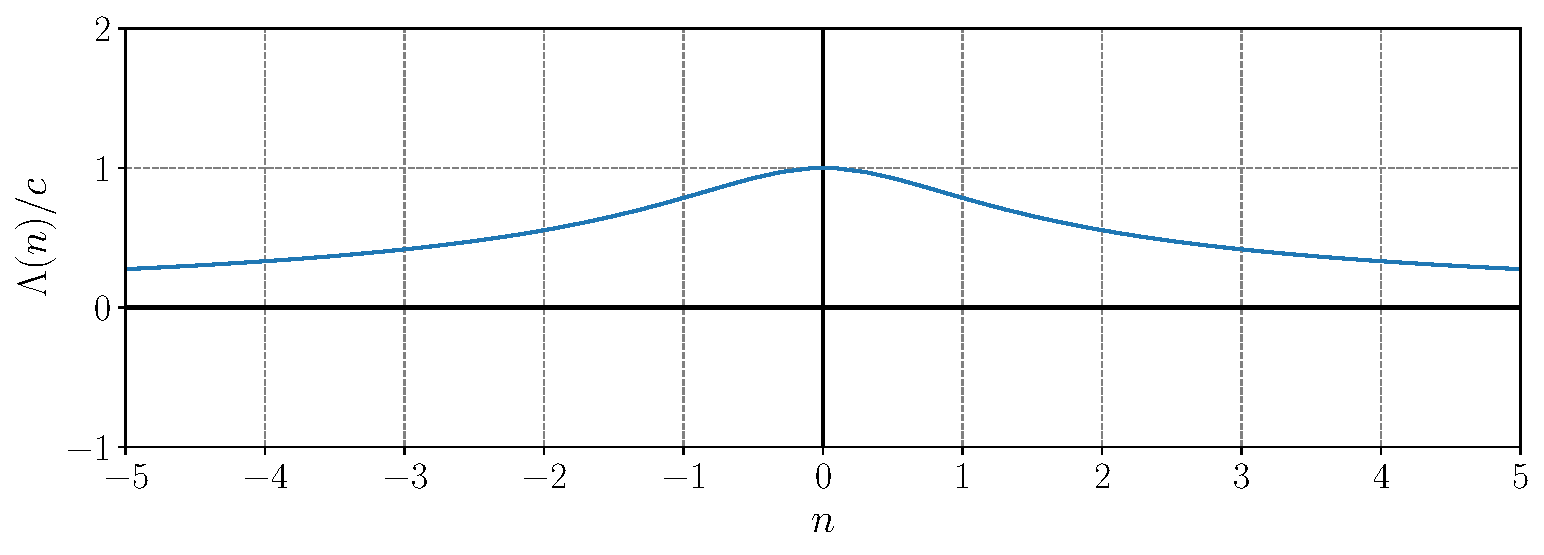
\includegraphics[width=0.75\textwidth]{images/lambda_function}
    \caption{$\Lambda(n)$ normalized by $c = \Sigma_s/\Sigma_t$.\label{fig:lambda}}
  \end{figure}

    \note{
      \begin{itemize}      
      \item If we plug this back into our previous equation and do a
        large amount of manipulation, we get a fairly simple
        relationship between the integrated error in one step to the
        integrated error in the previous step.
      \item This lambda function is maximized when $n = 0$. The lowest
        frequency error converges the slowest, and at a rate
        proportional to $\Sigma_s/\Sigma_t$.
      \end{itemize}
      
      }
}

\frame[c]{\frametitle{Conclusion}

\begin{block}{Conclusion}
  In the presence of a substantial scattering cross-section,
  source-iteration can converge arbitrarily slow because the error in
  diffuse, persistent modes after each iteration reduces by a factor
  of $\Sigma_s/\Sigma_t$.
\end{block}
\pause
Some acceleration schemes that have been developed to mitigate this issue:
\begin{itemize}
\item Diffusion synthetic acceleration (DSA).
\item Diffusion and transport two-grid methods (TG, TTG).
\end{itemize}
\pause
\begin{block}{Note}
  This is not the only portion of the transport solve that
  acceleration schemes are developed for.
\end{block}


\note{ This motivates the development of acceleration schemes to speed
  up this convergence. This is especially applicable to shielding
  problems where scattering is dominant, and reactors with a large
  amount of scattering

  You'll notice these use diffusion, because the diffusion equation
  will be good at calculating these large diffuse errors that are not
  coupled to space.
}
}

\section{Analyzing Acceleration}

\begin{frame}
  \frametitle{What is Acceleration?}
  \pause
  For an method to \textit{accelerate} the solve, it must remove more
  error from the solution for less work. Defining \textit{work} is
  challenging. In general, we use inversions of the transport matrix
  (or \textit{sweeps}) as a unit of work.
  \pause
\only<2->{
  \begin{figure}[H]
    \centering
    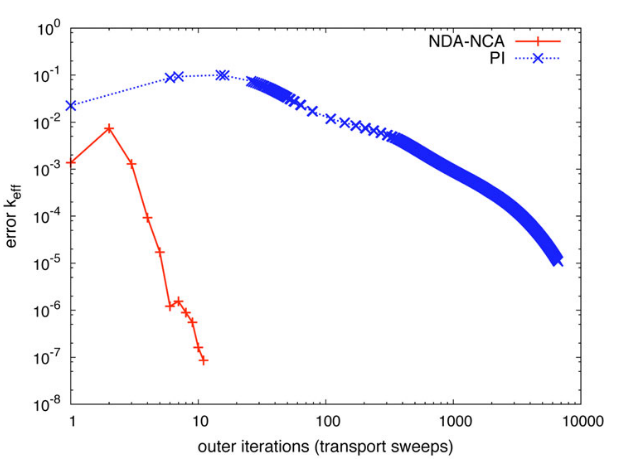
\includegraphics[width=0.5\textwidth]{images/nda_convergence_park}
    \caption{NDA convergence vs standard power iteration~\cite{Park2012}\label{fig:nda_convergence}}
  \end{figure}}

\note{
  The problem with this is that it's unclear how much actual work is
  being done in each step. You could form an acceleration scheme that
  solves in a single outer iteration, but is doing so
  \textit{actually} accelerating removing more error in less work, or
  just moving work around?

  We can use Fourier analysis like before, but things get complicated
  when we move into multidimensional problems, and start combining
  accelerating schemes. We need more insight into the acceleration process.
  }
\end{frame}

\frame{
  \frametitle{Analysis Challenges}
  \begin{figure}[H]
    \centering
    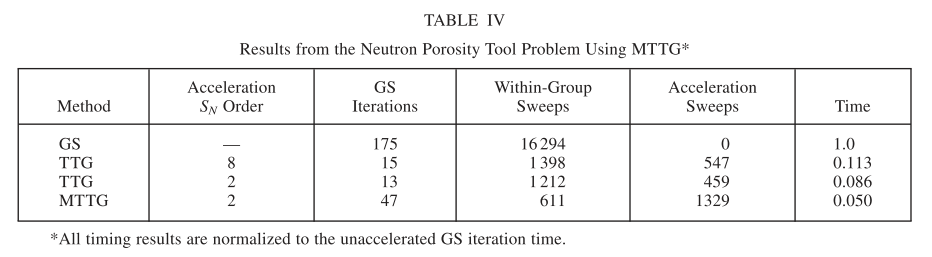
\includegraphics[width=\textwidth]{images/iteration_table}
    \caption{Iteration results table.~\cite{Evans2010}\label{fig:iteration_table}}
  \end{figure}

  \note{
    Here is an example of an iteration table from a paper analyzing
    the two-grid method. It shows both Gauss-Seidel iterations, within
    group sweeps and acceleration sweeps, but we don't have a clear
    idea of what parts of the problem are doing all the work. We don't
    know where the error is being removed, and if this method is doing
    it more economically or just shifting it around. The \textit{time}
    is a good indication, but not ideal. Is it proper to use clock
    time? CPU Time? How do we know that it's not faster because of
    better computer science. We not only need insight into the inner
    workings of acceleration schemes, but we need to dis-aggregate the
    computer science from the mathematics.
  }
  
}

\begin{frame}
  \frametitle{Analysis Challenges}
  A few challenges when analyzing the effectiveness of acceleration
  schemes include:
  \begin{itemize}[<+->]
  \item Work definition requires assumptions about algorithm efficiency.
  \item Combined or complex schemes may invalidate assumptions.
  \item Implementation and reproducibility can be difficult.
  \end{itemize}
  
  \note{
  \begin{itemize}
  \item Our definition of work is based on assumptions about
    algorithmic efficiency of the entire transport solve.
  \item Combining or using complex acceleration schemes may invalidate
    these assumptions.
  \item Implementing new schemes can be complicated, making it
    difficult to dis-aggregate implementation from theory. 
  \item It can be difficult to reproduce results when accelerated
    codes are not portable.
  \end{itemize}
    }
  
  \end{frame}

\begin{frame}
  \frametitle{Project Motivation}
  \begin{block}{Project}
    To create a novel tool that addresses these challenges, and acts
    as a laboratory for researchers to develop, test, and analyze
    acceleration schemes. 
  \end{block}

  This tool will provide a laboratory for researchers that:
  \begin{itemize}[<+->]
  \item Provides a controlled environment to run experiments.
  \item Provides analysis tools to make informed decisions about the
    results.
  \item Acts as a testing ground for new methods.
  \item Produces code that is portable, reproducible, and testable.
  \end{itemize}

  \note{
    \begin{itemize}
    \item Enables a controlled environment to test methods.      
    \item Acts as a testing ground for new methods for production codes.
    \end{itemize}

    }
  
  \end{frame}

  \section{BART}

\frame{
  \frametitle{Design Goals for BART}

  The Bay Area Radiation Transport (BART) is the new code in
  development with design goals to meet these needs. These goals include:
  
  \begin{enumerate}
  \item<1-> Leverage an object-oriented language and polymorphism.
  \item<2-> Include analysis tools.
  \item<3-> Provide a framework for experimentation.
  \item<4-> Utilize modern coding and tests practices.
  \end{enumerate}

  \note{
    \begin{itemize}
    \item Use object oriented programming and polymorphism to make it
      easier to implement new methods, and to limit the code needed to
      do so.
    \item Include enough tools to allow researchers to analyze the effectiveness of
      acceleration schemes.      
    \item Provide an framework for users to experiment with
    novel combinations of and modifications to existing acceleration
    schemes.
  \item Utilize modern coding and tests practices to make it
    easier for users to develop and have confidence in their solutions.
    \end{itemize}

    }
}

\begin{frame}
  \frametitle{Polymorphism}
  \begin{figure}[H]
    \centering
    \only<1>{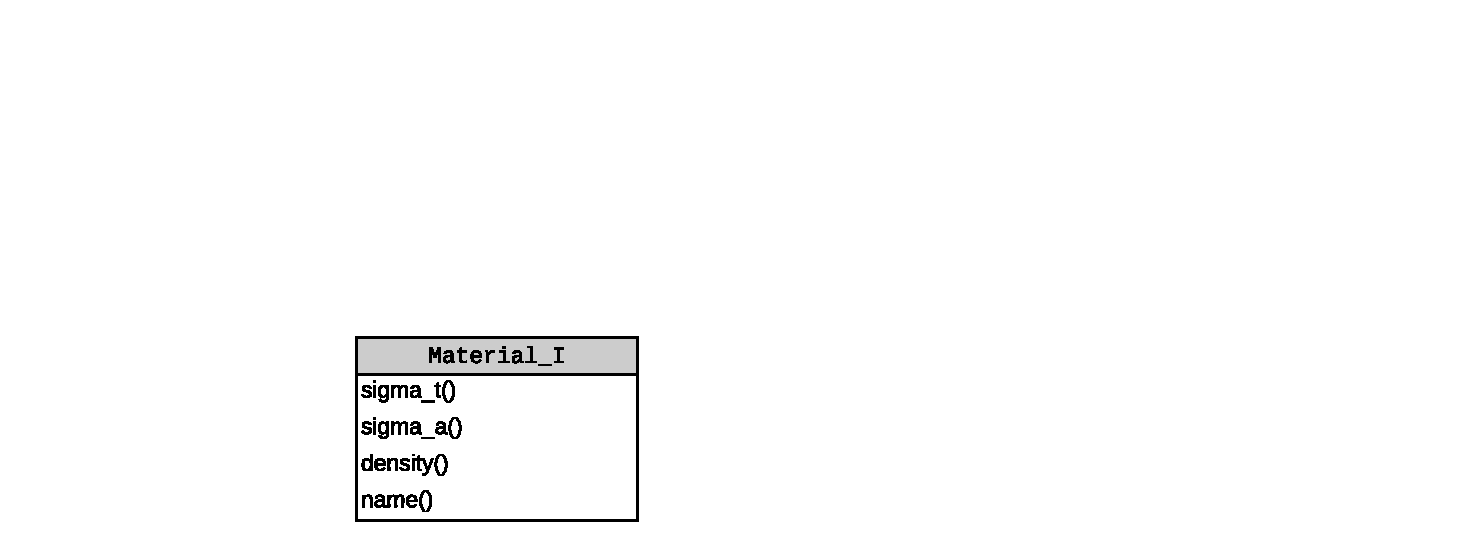
\includegraphics[width=\textwidth]{images/poly_1}}
    \only<2>{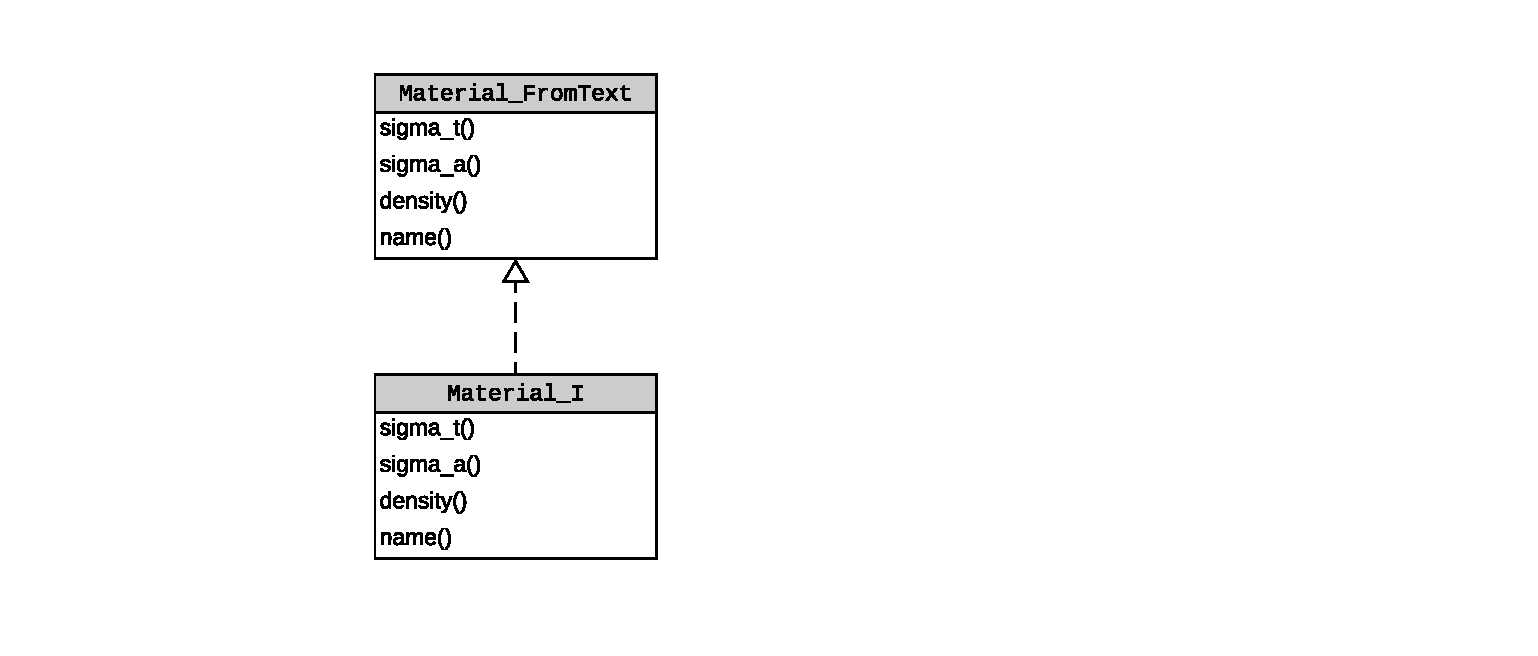
\includegraphics[width=\textwidth]{images/poly_2}}
    \only<3>{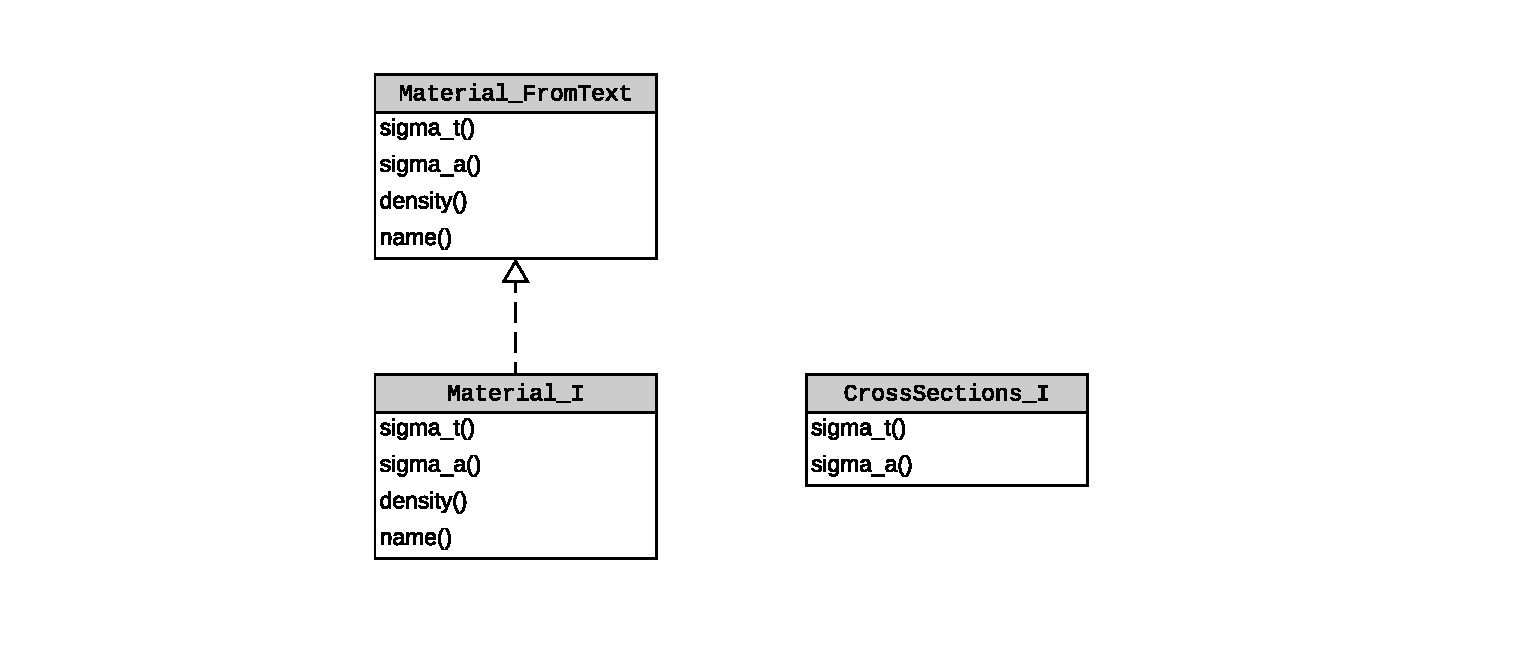
\includegraphics[width=\textwidth]{images/poly_3}}
    \only<4>{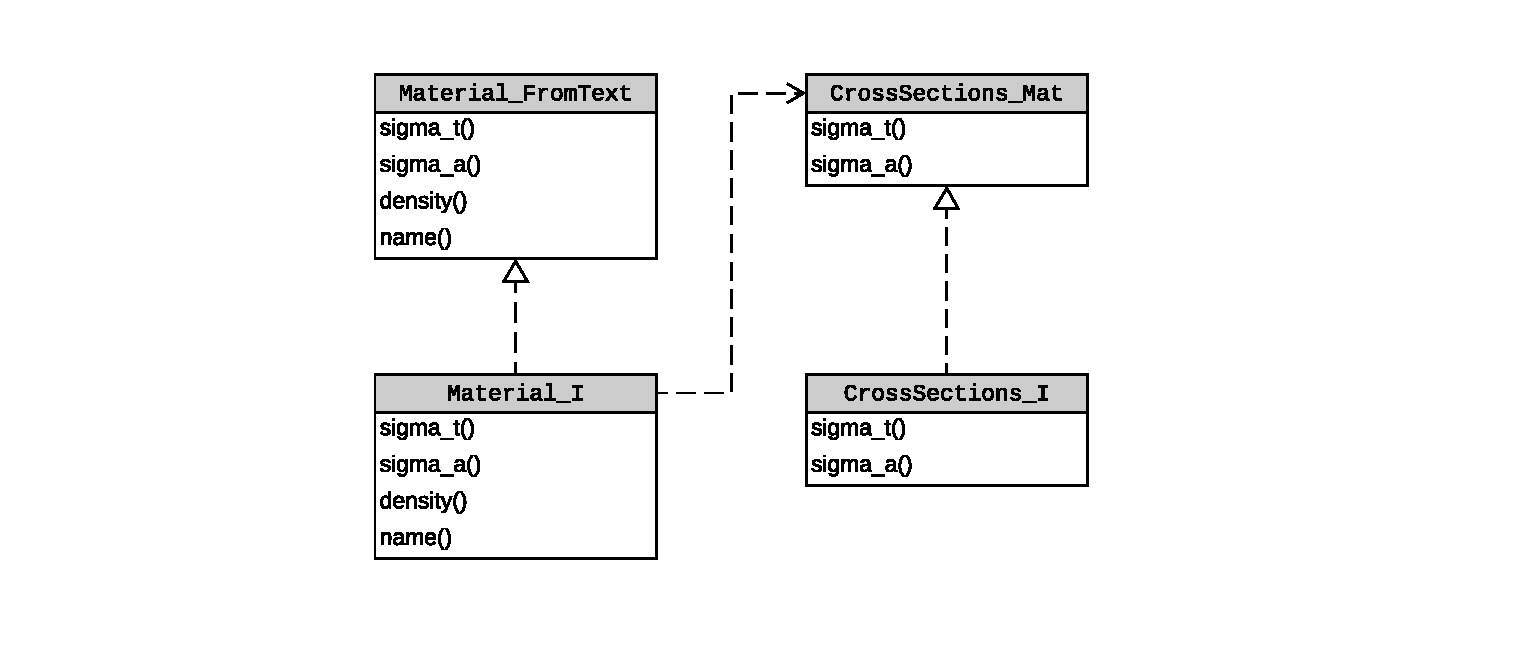
\includegraphics[width=\textwidth]{images/poly_4}}
    \only<5>{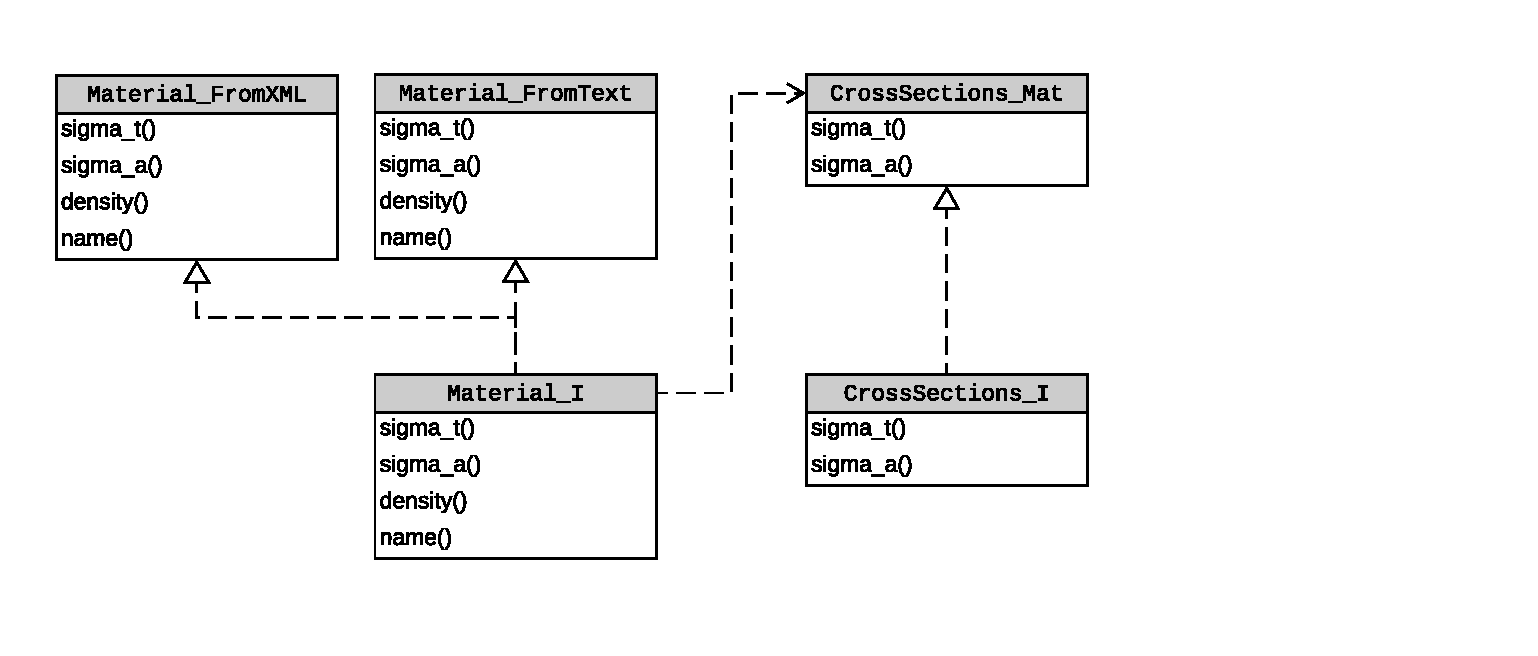
\includegraphics[width=\textwidth]{images/poly_5}}
    \only<6>{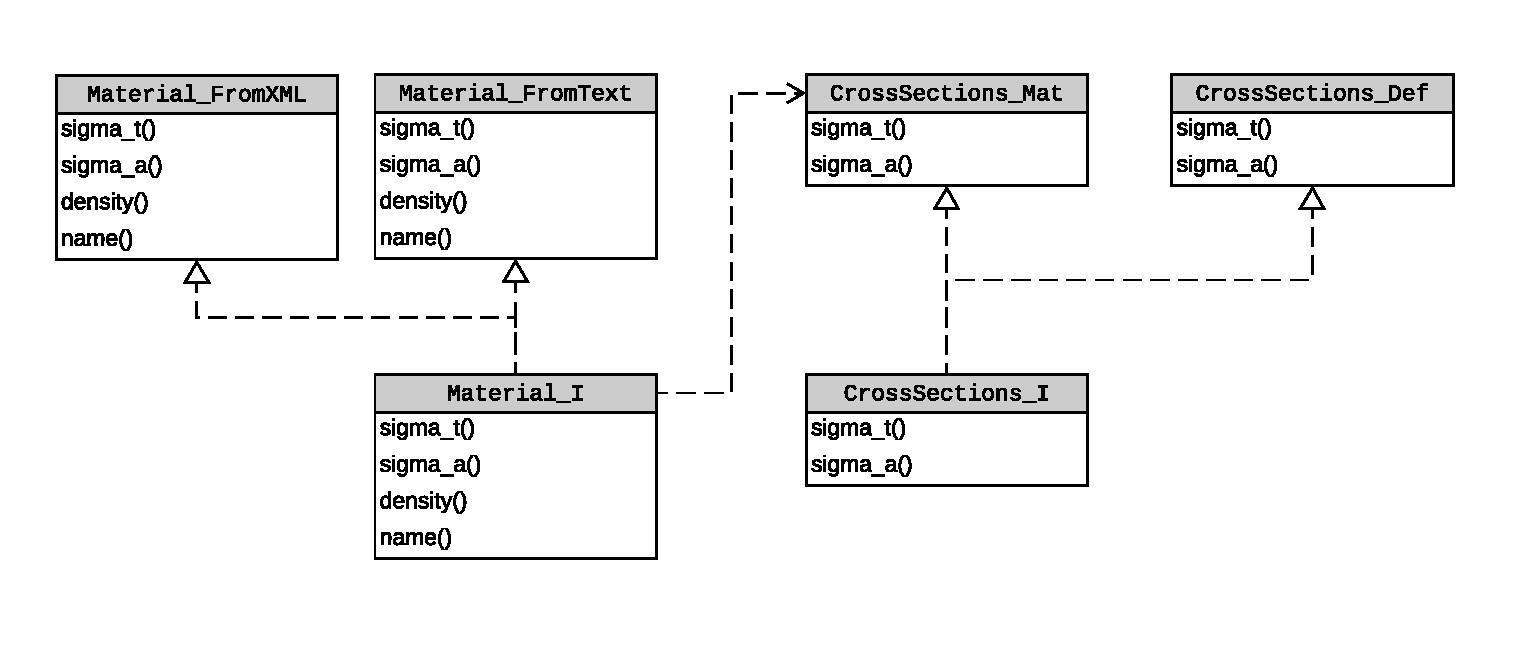
\includegraphics[width=\textwidth]{images/poly_6}}
  \end{figure}  
\end{frame}

\begin{frame}
  \frametitle{Polymorphism}
  \begin{figure}[H]
    \raggedright
    \only<1>{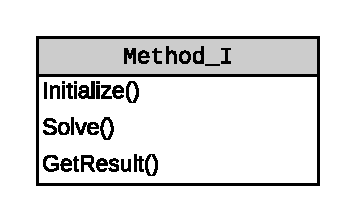
\includegraphics[scale=0.55]{images/poly_min_1}}
    \only<2>{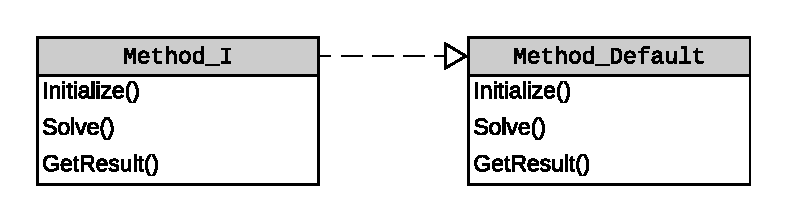
\includegraphics[scale=0.55]{images/poly_min_2}}
    \only<3->{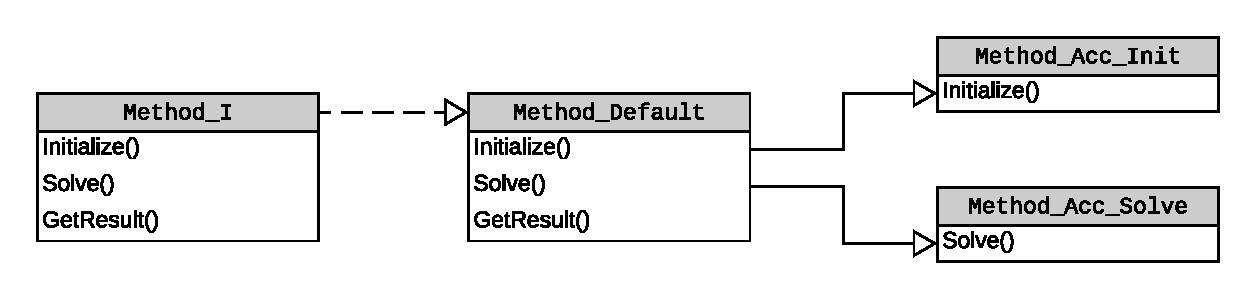
\includegraphics[scale=0.55]{images/poly_min_3}}
  \end{figure}
  \only<4->{
  }
\end{frame}

\begin{frame}
  \frametitle{Polymorphism Benefits}
  The use of polymorphism in BART
  \begin{itemize}
  \item<1-> Minimizes code changes needed to implement new methods,
    making it faster and easier.
  \item<2-> Enables a true comparison of the accelerated solve to a
    control solve.
  \item<3-> Makes the modifications \textit{portable}.    
  \item<4-> Enables us to compare the implementation of the method to
    dis-aggregate the computer science from the method itself.
  \end{itemize}
 
\end{frame}

\begin{frame}
  \frametitle{Instrumentation}
  \begin{block}{Goal 2}
    Include tools to analyze the effectiveness of
    acceleration schemes.
  \end{block}
  \pause BART will include the ability to \textit{instrument} a solve
  to gather enough data to draw useful conclusions about the effectiveness of
  acceleration schemes.  \pause
\begin{itemize}[<+->]
  \item Storage of solve parameters (eigenvalues, fluxes).
  \item Storage of hierarchy of iterations.
  \item Calculation and storage of error or residual.
  \item Analysis of Fourier error modes coefficients.
  \end{itemize}

 \onslide<+->{
  \begin{block}{}
    Adding new instrumentation must be easy!
  \end{block}}
\end{frame}

\begin{frame}
  \frametitle{Framework for experimentation}
  \only<1>{
  \begin{block}{Goal 3}
    Provide a framework for users to experiment with
    novel combinations of and modifications to existing acceleration
    schemes.
  \end{block}}
\only<2>{
  \begin{figure}[H]
    \centering
    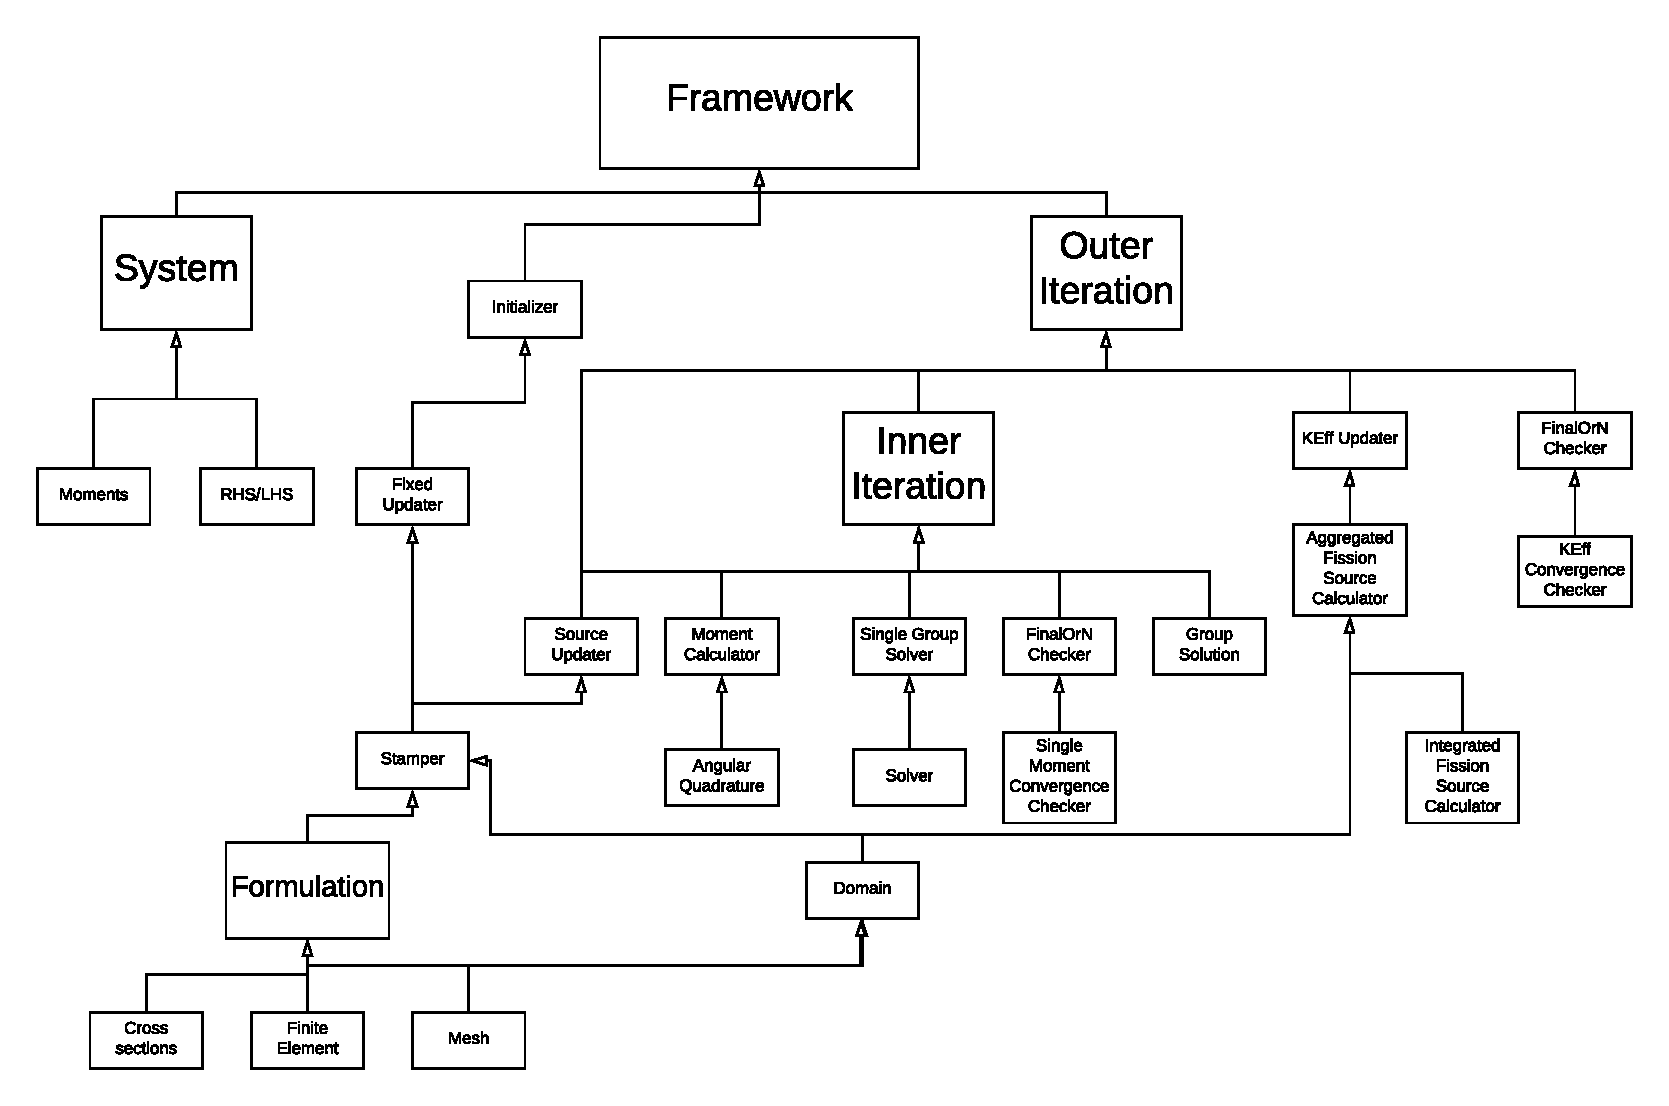
\includegraphics[width=0.9\textwidth]{images/bart}
  \end{figure}
  }
\end{frame}

\begin{frame}
  \frametitle{Modern Coding Practices}
  \begin{block}{Goal 4}
    Utilize modern coding and tests practices to make it
    easier for users to develop and have confidence in their solutions.
  \end{block}
  \begin{itemize}
  \item Build using the methods of modern \texttt{C++-14}.
  \item BART uses the \texttt{googletest} and \texttt{googlemock}
    libraries for unit testing. Unit testing coverage via \texttt{codecov}
  \item All dependencies for BART are built in an available Docker
    container.
  \item Continuous integration via \texttt{travis.ci}.
  \end{itemize}  
    
\end{frame}

\begin{frame}
  \frametitle{Protocol Buffers}
  Cross-sections can be stored in a novel protocol buffer format.
  \begin{columns}
    \begin{column}{0.5\textwidth}
      \pause
      Benefits:
  \begin{itemize}[<+->]
  \item Structured data format.
  \item Automatic generation of parsing code.
  \item Very fast parsing and small file size.
  \end{itemize}
\end{column}
\begin{column}{0.5\textwidth}  %%<--- here
    \begin{center}
     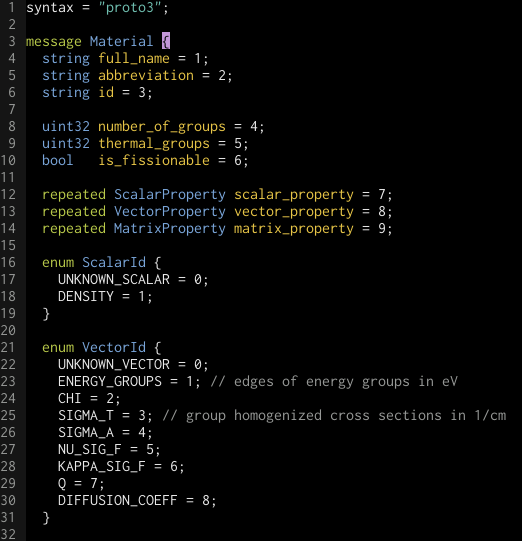
\includegraphics[width=\textwidth]{images/protocol_buffer}
     \end{center}
\end{column}
\end{columns}

  

    
\end{frame}

\begin{frame}
  \frametitle{Project Deliverables}

  \begin{enumerate}[<+->]
  \item A new \texttt{C++} code that solves the transport
    equation using continuous finite-element methods.
  \item A new cross-section and material storage method using protocol buffers.
  \item Implementation of a novel acceleration method.
  \item A novel analysis of this acceleration methods using
    instrumentation implemented in the code.
  \end{enumerate}
\end{frame}

\section{The $S_N$ equations}

\frame[c]{\frametitle{The multigroup $S_N$ equations}
  Apply the following discretizations:
  \begin{itemize}
  \item<1-> Apply a Petrov-Galerkin scheme in energy (multigroup
    method), splitting into $G$ coupled equations.
  \item<2-> Apply a collocation scheme in angle, solving at angles $\oh_a$.
  \item<3-> Expanding scattering cross-section in Legendre Polynomials
    with a maximum degree $N$.
  \end{itemize}

  \only<3>{
      \begin{equation*}
    \Sigma_{s,g'g,\ell} =
    \int_{-1}^{1}\Sigma_{s,g'g}(\rvec,\mu)P_{\ell}(\mu)d\mu, \quad \mu
    = \oh' \cdot \oh
  \end{equation*}
  \begin{equation*}
    \phi_{g, \ell, m} = \int_{4\pi}\phi_g(\rvec, \oh')Y_{\ell, m}(\oh')d\oh'
  \end{equation*}
}
\onslide<4->{
  \pause
  \begin{block}{Multigroup $S_N$ equations}\vspace{-0.25cm}
    \begin{align*}
      &\left[\oh_a \cdot \nabla + \Sigma_{t,g}(\rvec)\right]\psi_g(\rvec,
        \oh_a) \\
      & \quad \quad = \sum_{g' = 0}^{G}\sum_{\ell = 0}^N\sum_{m =-\ell}^{\ell}\Sigma_{s,g'g,\ell}
        Y_{\ell,m}(\oh_a)\phi_{g',\ell, m}(\rvec) + Q_g(\rvec, \oh_a)
    \end{align*}
  \end{block}
  }
  \note{
    \begin{itemize}      
    \item Multigroup method splits the equations into $G$ coupled equations
    \item Collocation scheme in angle uses points for a quadrature
      rule for integrating angular flux to get flux moments
    \item Expand in Legendre polynomials, use polynomial addition theorem,
    \end{itemize}
    }
  }
  
\frame[c]{\frametitle{Iterative Solving Methods}
  Expressed in operator form, this is
  \begin{align*}
    \mat{L}_g\mat{\Psi}_g = \mat{M}\sum^{G}_{g' = 0}\mat{S}_{g'  g}\mat{\Phi}_{g'}
    + \mat{Q}_g, \quad \mat{\Phi}_{g} = \mat{D}\mat{\Psi}_g\;.
  \end{align*}
  \pause
  Splitting the scattering source into down-scattering and up-scattering terms,
  \begin{align*}
    \mat{L}_g\mat{\Psi}_g = \mat{M}\sum^g_{g' = 0}\mat{S}_{g' 
    g}\mat{\Phi}_{g'}
    + \mat{M}\sum^G_{g' = g+1}\mat{S}_{g'  g}\mat{\Phi}_{g'}
    + \mat{Q}_g\;,
  \end{align*}
  \pause
  And holding the source $\mat{Q}$ fixed leads to a Gauss-Seidel (scattering) source iteration,
    \begin{align*}
    \mat{L}_g\mat{\Psi}^{k+1}_g = \mat{M}\sum^g_{g' = 0}\mat{S}_{g' 
    g}\mat{\Phi}^{k+1}_{g'}
    + \mat{M}\sum^G_{g' = g+1}\mat{S}_{g'  g}\mat{\Phi}^k_{g'}
    + \mat{Q}_g\;.
    \end{align*}
    \note{
      \begin{itemize}
      \item M is the moment-to-discrete, D is the reverse
      \item Important to note that the $G$-th energy group is the
        lowest.        
      \end{itemize}
      }     
    }

\frame[c]{\frametitle{Iterative Solving Methods}
  For a multiplying-medium problem, the fixed source $\mat{Q}$ is
  replaced with the fission source,
  \begin{align*}
    \mat{L}_g\mat{\Psi}_g = \mat{M}\sum^{G}_{g' = 0}\left[\mat{S}_{g'  g}\mat{\Phi}_{g'}
    + \frac{1}{k}\mat{F}
    _{g'}\mat{\Phi}_{g'}\right]\;.
  \end{align*}
  Holding the scattering source fixed leads to power iteration
  (fission source iteration),
  \begin{align*}
    \mat{L}_g\mat{\Psi}^{k+1}_g = \mat{M}\sum^{G}_{g' = 0}\left[\mat{S}_{g'  g}\mat{\Phi}^{0}_{g'}
    + \frac{1}{k}\mat{F}_{g'}\mat{\Phi}^{k}_{g'}\right]\;.
  \end{align*}
  In general, to converge both the fission and scattering sources,
    power iteration is paired with source iteration in an inner-outer
    convergence scheme.
  }

\frame[c]{\frametitle{Convergence Challenges}

\begin{block}{Convergence of Source Iteration}
  Gauss-Seidel source iteration can converge arbitrarily slow as
  $\Sigma_s/\Sigma_t$ approaches unity.
\end{block}
\pause
\begin{block}{Convergence of Power Iteration}
  Power iteration can convergence arbitrarily slow as the dominance
  ratio $k_1/k_0$ approaches unity.
\end{block}

\onslide<+->{
Different acceleration schemes address different issues:
\begin{itemize}[<+->]
\item Power Iteration: Nonlinear diffusion acceleration (NDA).
\item Source Iteration: Diffusion two-grid method (TG).
\item Both: A novel combination of NDA and TG.
\end{itemize}
}
}

\section{Acceleration Methods}

\frame[c]{\frametitle{Nonlinear Diffusion Acceleration (NDA)}
  \begin{block}{Big Idea}
    Accelerate power iteration by using a diffusion solve in place of
    the standard transport equation source iteration~\cite{Park2012}.
  \end{block}

  Couples an angular solve with a diffusion solve and,
  \begin{itemize}
  \item Uses the angular solve to improve accuracy of diffusion
    solve via current.
  \item Uses the diffusion solve to improve accuracy of angular solve
    via scalar flux.
  \end{itemize}
}



\frame[c]{\frametitle{Nonlinear Diffusion Acceleration (NDA)}
\pause
  Start, with the single-group first-order transport
  equation~\cite{Park2012, Hammer2017}, and integrate over angle:
  \begin{equation*}
    \nabla \cdot J_g + \left(\Sigma_{t,g} - \Sigma_s^{g\to g}\right)
    \phi_g = \sum_{g' \neq g}\Sigma_s^{g' \to g}\phi_{g'} + q_g,\quad J_g \equiv \int
    d\oh \oh \psi_g(\oh)\;.
  \end{equation*}
  \pause
  As a closure to this problem, it is common to define current using \textit{Fick's law},
  \begin{equation*}
    J_g = -D\nabla \phi_g\;.
  \end{equation*}
  \pause
  Construct an additive correction to the current using information
  from an angular solve:
  \begin{align*}
    J_g &= -D\nabla \phi_g + J_g - J_g\\
        &= -D\nabla \phi_g + \int_{4\pi}d\oh\oh\psi_g +
          D\nabla\phi_g
  \end{align*}
  
  \note{
    \begin{itemize}
    \item Uses a lower order diffusion solve to accelerate a higher
    order solve. 
  \item Start with the same single-group first-order
    transport equation, multiply by and integrate over angle, giving the
    ``neutron continuity equation.''
  \item We need closure for this problem, so often we use Fick's law,
    we will introduce a correction onto Fick's Law based on a higher
    order solve.
  \item We will introduce an additive correction based on our two
    definitions of the current.
    \end{itemize}
}
}

\frame[c]{\frametitle{Nonlinear Diffusion Acceleration (NDA)}
  Fold the additive correction into a \textit{drift-diffusion vector}:
  \begin{align*}
    J_g &= -D\nabla \phi_g + \int_{4\pi}d\oh\oh\psi_g +
          D\nabla\phi_g \\
        &= -D\nabla\phi_g + \left[\frac{\int_{4\pi}d\oh\oh\psi_g +
          D\nabla\phi_g}{\phi_g}\right]\phi_g \\
        &= -D \nabla \phi_g + \hat{D}_g\phi_g\;.
  \end{align*}
  %\pause
  Plugging this into our integrated transport equation gives the
low-order non-linear diffusion acceleration equation (LONDA),
  \begin{block}{}
    \begin{equation*}
      \nabla\cdot\left[-D\nabla + \hat{D}_g\right]\phi_g +
      \left(\Sigma_{t,g} - \Sigma_s^{g \to g}\right)\phi_g = \sum_{g' \neq g}\Sigma_s^{g' \to g}\phi_{g'} + q_g
    \end{equation*}
  \end{block}

  
  \note{
    \begin{itemize}
    \item We combine these corrections into a drift diffusion vector.
    \item This gives us the LONDA equation, which is just the same
      integrated transport equation with a corrected current term.
    \item Presumably, the ``higher order'' angular solve will have
      better current information, so we can use it to calculate the drift diffusion vector.
    \end{itemize}
  }
}

\frame[c]{\frametitle{NDA algorithm}
  \begin{figure}[H]
    \centering
    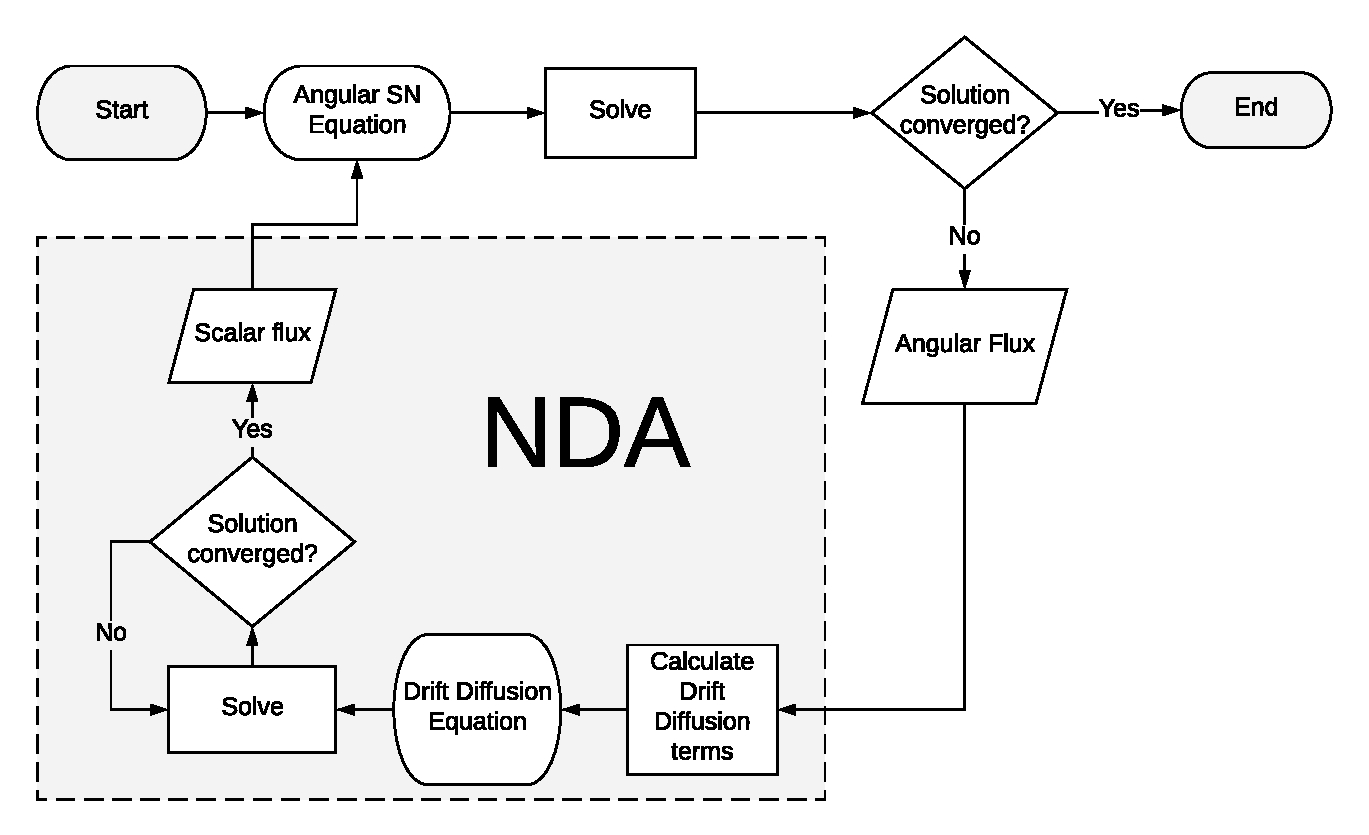
\includegraphics[width=\textwidth]{images/nda_flowchart}
    \caption{NDA Algorithm.\label{fig:nda_algorithm}}
  \end{figure}

  \note{
    \begin{itemize}
    \item NDA algorithm showing inner low order loop, and outer high
      order loop.
    \item In general, outer loop updates both scattering and fission
      source, checking for $k$ convergence. Inner loop updates
      fission source, also checking $k$ convergence.
    \end{itemize}
  }
}
    
\frame[c]{\frametitle{Two-grid acceleration}

To mitigate convergence issues in source-iteration Adams and Morel~\cite{Adams1993} developed the
two-grid method which rests on two assumptions:
\begin{itemize}
\item<1-> The persistent error modes can be accurately determined by a
  coarse-grid approximation.
\item<2-> Solving this coarse-grid approximation is more economical
  than solving the actual equation.
\end{itemize}
\onslide<3->{
\begin{block}{Two-grid Acceleration}
  Solve for the error using a coarse-grid approximation, and use it as
  a correction to our solution in each step.
\end{block}}



\note{
  \begin{itemize}
  \item This should speed up the solve by giving an addition reduction
    in those diffuse persistent error modes.
  \end{itemize}
  }
}
    
\frame[c]{\frametitle{Two-grid acceleration}
  Step 1: Solve the angular $S_N$ source-iteration equation,
  \begin{align*}
    \mat{L}_g\mat{\Psi}^{i+\frac{1}{2}}_g = \mat{M}\sum^g_{g' = 0}\mat{S}_{g' 
    g}\mat{\Phi}^{i+\frac{1}{2}}_{g'}
    + \mat{M}\sum^G_{g' = g+1}\mat{S}_{g'  g}\mat{\Phi}^k_{g'}
    + \mat{Q}_g\;.
  \end{align*}
  Step 2: Calculate the isotropic component of the residual,
  \begin{align*}
    \mat{R}^{i + \frac{1}{2}}_{g, 0} = \sum_{g' =
    g+1}^{G}\mat{S}_{g'g}\left(\mat{\Phi}^{i + \frac{1}{2}}_{g'} - \mat{\Phi}^{i}_{g'}\right)
  \end{align*}
  Step 3: Calculate the error.
    \begin{align*}
      \mat{L}_g\mat{\epsilon}^{i+\frac{1}{2}}_g = \mat{M}\sum^G_{g' = 0}\mat{S}_{g' 
    g}\mat{\varepsilon}^{i+\frac{1}{2}}_{g'}
    + \mat{R}_g^{i+\frac{1}{2}}
    \end{align*}
  }

\frame[c]{\frametitle{Two-grid acceleration}\

  Step 3a: Calculate error using integrated diffusion approximation.
      \begin{equation*}
      \left(-\nabla \cdot \left<D_g\right> \nabla  +
        \Sigma_g\right)\tilde{\varepsilon}_g^{i+\frac{1}{2}} = \sum_{g' =
        0}^G\Sigma_{s,g'g,0}\tilde{\varepsilon}_{g'}^{i+\frac{1}{2}} + \mat{R}^{i+\frac{1}{2}}_{g,0}
    \end{equation*}

    Step 4: Correct the flux
    \begin{equation*}
      \mat{\Psi}_g^{i+1} = \mat{\Psi}_g^{i+ \frac{1}{2}} + \mat{M}\tilde{\varepsilon}_{g}^{i+\frac{1}{2}}
    \end{equation*}

This will accelerate our solution only if it removes more error with
less work than our original method.
    
}

\frame[c]{\frametitle{Two-grid Acceleration}

  \begin{figure}[H]
    \centering
    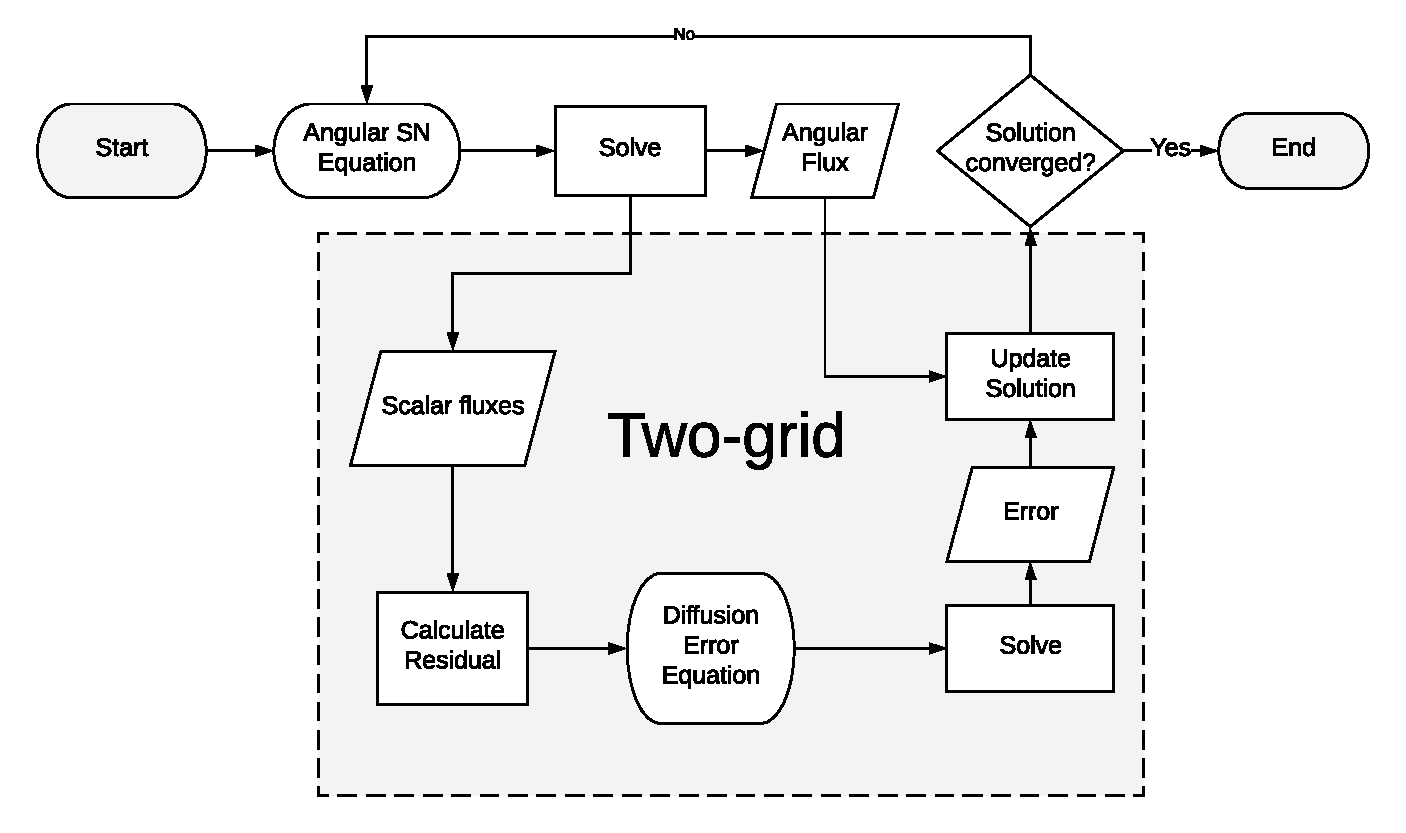
\includegraphics[width=0.9\textwidth]{images/two_grid_flowchart}
    \caption{Two-grid flowchart.\label{fig:two_grid_algorithm}}
  \end{figure}

}  
   

\frame[c]{\frametitle{Acceleration Methods}
  Two acceleration methods:
  \begin{itemize}
      \item \textbf{Nonlinear Diffusion Acceleration}: improves the
    convergence of the multi-group Gauss-Seidel iteration, but suffers
    from convergence issues with a large amount of upscattering.
  \item \textbf{Two-grid Acceleration}: improves the convergence of
    multi-group problems with a large amount of upscattering.
  \end{itemize}
  
  \begin{block}{Novel Combination}
    Use two-grid acceleration to improve the convergence rate of the
    low-order portion of the NDA solve.
  \end{block}
}

\frame[c]{\frametitle{Combining Acceleration Methods}
  \begin{figure}[H]
    \centering
    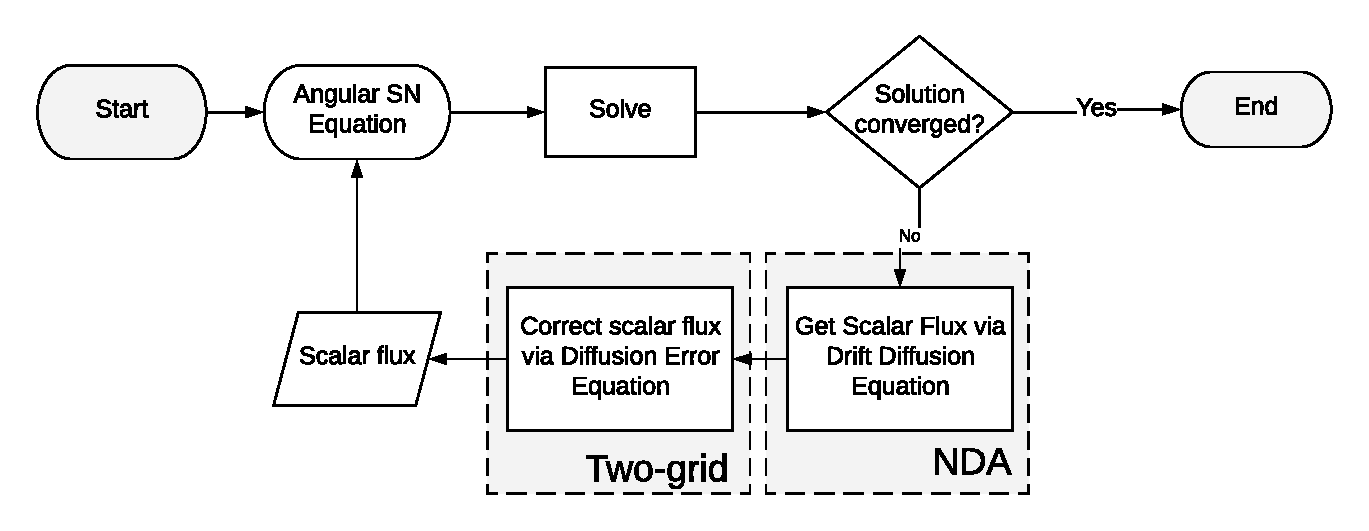
\includegraphics[width=\textwidth]{images/nda_two_grid}
    \caption{Two-grid flowchart.\label{fig:two_grid_algorithm}}
  \end{figure}
}

  

\section{Plan and Future Work}

\frame[label=IMPLEMENTATION]{\frametitle{BART Implementation Plan}

  \onslide<1->{
  Formulations: 
  \begin{itemize}
  \item Interface for \hyperlink{SECOND_ORDER}{second-order} transport equation formulations
    using continuous finite element methods.
  \item Implementation of Diffusion.
  \item Implementation of Self-Adjoint angular flux equation.
  \end{itemize}
  }

  \onslide<2-> {
  Acceleration methods:
  \begin{itemize}
  \item Nonlinear diffusion acceleration.
  \item Two-grid acceleration.
  \item Nonlinear diffusion acceleration with two-grid acceleration.
  \end{itemize}
}

\onslide<3-> {
  Instrumentation:
  \begin{itemize}
  \item In-step Fourier-transform.    
  \item Iteration hierarchy counting.
  \item Automated runs based on mesh refinement.
  \end{itemize}
  }
}

\begin{frame}
  \frametitle{Future Work}
  \begin{itemize}[<+->]    
  \item Addition of Discontinuous-Galerkin Finite Element Formulations support
    to BART.\@
  \item More acceleration methods implemented to test different combinations.
  \item Better or more complex \textit{in situ} analysis of acceleration efficiency.
  \item Automated acceleration control (adaptive acceleration).
  \end{itemize}
\end{frame}

\begin{frame}[noframenumbering, plain]
  \vfill
  \centering
  Thank you for your time!
  \vfill
\end{frame}


\frame[noframenumbering, plain]{\frametitle{References}
\tiny{\bibliographystyle{plain}}
\bibliography{bib/bib}
}

\appendix

\section{Backup Slides}

\frame[c]{\frametitle{Energy discretization}
  Introduce a discretization of the energy domain $\mathbb{E}$ into $G$
  non-overlapping elements, such that
  \begin{align*}
    E_h = \left\{E_1, E_2, \ldots, E_G\right\}, \quad \mathbb{E} = \bigcup_{g=1}^GE_g
  \end{align*}
  
  Assume that the energy-dependent angular flux can be separated into
  a group angular flux and a energy function within each of
  these groups
  \begin{align*}
    \psi(\rvec, E, \oh) \approx \psi_g(\rvec, \oh)f_g(E), \quad E \in E_g 
  \end{align*}

  This gives us $G$ coupled equations for each energy group,
  converting the integral scattering term into a summation,
  \begin{equation*}
    \left[\oh\cdot  \nabla +
      \Sigma_{t,g}(\rvec)\right]\psi_g(\rvec,\oh) = \sum_{g' = 0}^G\Sigma_{s,g'\to g}(\rvec, \oh' \to
  \oh)\psi_{g'}(\rvec,\oh') + Q_g(\rvec, \oh)\;.
  \end{equation*}

  \note{
    \begin{itemize}
    \item Say that the function $f_g$ is zero inside element, and 0
      outside, Petrov-Galerkin scheme.
    \end{itemize}
    
    }
  }

\frame[c]{
  \frametitle{Iterative Solve Error}
  \onslide<1->{Much of our analysis will require an examination of the error in
  each step of an iterative method. This is found by subtracting our
  method from the original equation.}
  \only<2>{
  \begin{align*}
    \mat{L}_g\mat{\Psi}_g &= \mat{M}\sum^g_{g' = 0}\mat{S}_{g' 
    g}\mat{\Phi}_{g'}
    + \mat{M}\sum^G_{g' = g+1}\mat{S}_{g'  g}\mat{\Phi}_{g'}
    + \mat{Q}_g \\
    \mat{L}_g\mat{\Psi}^{i+1}_g &= \mat{M}\sum^g_{g' = 0}\mat{S}_{g' 
    g}\mat{\Phi}^{i+1}_{g'}
    + \mat{M}\sum^G_{g' = g+1}\mat{S}_{g'  g}\mat{\Phi}^i_{g'}
    + \mat{Q}_g
  \end{align*}}
\onslide<3->{
  \begin{equation*}
    \mat{L}_g\mat{\epsilon}^{i+1}_g = \mat{M}\sum^g_{g' = 0}\mat{S}_{g' 
    g}\mat{\varepsilon}^{i+1}_{g'}
    + \mat{M}\sum^G_{g' = g+1}\mat{S}_{g'  g}\mat{\varepsilon}^i_{g'}
  \end{equation*}
  \begin{align*}
    \epsilon^{i+1}_{g} &= \mat{\Psi}_g - \mat{\Psi}_g^{i+1} \\
    \varepsilon^{i+1}_g &= \mat{D}\epsilon_g^{i+1}
  \end{align*}
}
}
  

\frame[c, label=SECOND_ORDER]{\frametitle{Second-order forms of the Transport Equation}
  There are various second-order, self-adjoint forms of the transport equation.
  \begin{itemize}
  \item Even/Odd-parity equations (EP).
  \item Weighted least-squared formulation (WLS).    
  \item Self-Adjoint angular flux (SAAF).
  \end{itemize}

  With advantages and disadvantages compared to the standard
  first-order forms. Advantages include:
  \begin{itemize}
  \item They can be solved on multidimensional finite element meshes
    using standard continuous finite element methods (CFEM).
  \item CFEM methods result in symmetric positive-definite (SPD)
    matrices.
  \item When using the $P_N$ formulation, the flux moments are
    strongly coupled via $\oh \cdot \nabla$.    
  \end{itemize}

  \note{
    \begin{itemize}
    \item First-order forms of the TE form block lower-triangular that
      can be swept. But on many meshes, there are slightly re-entrant
      cells that will break this pattern.
    \item Solution methods for SPD matrices are better, CG vs. GMRES.
    \end{itemize}

  }
}

\frame[c]{\frametitle{Second-order forms of the Transport Equation}
  Disadvantages include:
  \begin{itemize}
  \item<1-> CFEM methods result in a general sparse matrix, not a
    block lower-triangular.
  \item<2-> In some forms (EP), reflective boundary
    conditions have fully implicit coupling between incoming and
    outgoing flux. SAAF avoids this only coupling incoming to
    outgoing.
  \item<3-> Full angular flux can be hard to calculate for parity-forms.
  \item<4-> Difficulties with solving in voids (can be avoided using SAAF).
  \item<5-> Difficulties in a pure scattering media.
  \end{itemize}

  \note{
    \begin{itemize}
    \item Block lower-triangular would have allowed us to sweep.
    \item In pure scattering, there is a singularity in the scattering
      matrix for OP and SAAF in the spherical-harmonic basis. This is
      because it is diagonal and the first entry is $1/(\Sigma_t -
      \Sigma_{s0})$ which is $1/0$
    \end{itemize}
    }
  }

  \frame[c]{\frametitle{Self-adjoint angular flux equation (SAAF)}
  
 Start with the single-group first-order transport equation~\cite{Morel1999}:
  \begin{equation}
    \label{eq:single_group_for_saaf}
    \oh \cdot \nabla \psi + \Sigma_t \psi = S \psi + q\;.
  \end{equation}
  %\pause
Solve for $\psi$,
  \begin{equation*}
    \psi = \frac{1}{\Sigma_t}\left[S\psi + q - \oh \cdot \nabla \psi\right]\;,
  \end{equation*}
  and plug back into the gradient term in
  Eq.\ref{eq:single_group_for_saaf}.
    %\pause
  \begin{block}{}
    \begin{equation*}
    - \oh \cdot \nabla \frac{1}{\Sigma_t}\oh \cdot \nabla \psi +
      \Sigma_t \psi = S\psi + q - \oh \cdot \nabla \frac{S\psi +
        q}{4\pi}
    \end{equation*}
  \end{block}
  With boundary conditions, for all $\vec{r} \in \partial D$:
  \begin{equation*}
      \psi = f, \quad \oh
      \cdot \hat{n} < 0 
    \end{equation*}
\begin{equation*}
      \oh \cdot \nabla \psi + \Sigma_t\psi= S\psi + q, \quad \oh
      \cdot \hat{n} > 0 
    \end{equation*}
    \hyperlink{IMPLEMENTATION}{\beamergotobutton{Back to implementation}}
\note{The Self-adjoint angular flux equation (SAAF) is a second-order from
  of the transport equation introduced by Morel and McGhee in 1999. To
  derive, consider scattering term part of tte source. Properties of SAAF
  \begin{itemize}
  \item +Can solve using standard CFEM methods, which give SPD matrices
    (can use CG instead of GMRES)  
  \item +Full angular flux is obtained by solve (unlike Even/Odd
    parity)
  \item +BCs only coupled in one direction when reflective
  \item -General sparse matrix, not block lower-triangular (no
    sweeping)
  \item -Pure scattering causes issues like odd-parity
  \end{itemize}
}
}
 

\end{document}

%%% Local Variables:
%%% mode: latex
%%% TeX-master: t
%%% End:
